\documentclass[11pt]{article}
\usepackage{amsfonts,amsmath,amssymb,amsbsy,amsthm}
\usepackage{latexsym,bm}
\usepackage{upgreek}
\usepackage{graphics,graphicx}
\usepackage{subfigure}
\usepackage{subfigmat}
\usepackage{psfrag}
\usepackage{listings}
\usepackage{url}
\usepackage[square,numbers,comma,sort&compress]{natbib}
\usepackage{float}

\restylefloat{figure}

%macro for unnumbered aligned environments
\newcommand{\eq}[1]{\begin{align*}#1\end{align*}}

%macro for numbered equations
\newcommand{\eqn}[2]{
  \begin{equation}
    \label{#1}
    #2
  \end{equation}
}

\newcommand{\eps}{\epsilon}
\newcommand{\lam}{\lambda}

%macro for referencing equations
\newcommand{\eqr}[1]{eqn~(\ref{#1})}

%macro for frac partials
\newcommand{\fp}[2]{\frac{\partial#1}{\partial#2}}
\newcommand{\de}[2]{\frac{d #1}{d #2}}
\newcommand{\fpp}[2]{\frac{\partial^2 #1}{\partial#2^2}}

%macro for inline partials
\newcommand{\p}[1]{\partial_{#1}}

\newcommand{\mat}[2]{\left[\begin{array}{#1}#2\end{array}\right]}

\begin{document}
\begin{center}
{\large\bf 
Jeff Wendling\\
\today\\
Math 801\\
Final Exam
}
\end{center}
\begin{description}
\item[Problem 1]
We attempt to find an asymptotic approximation to
\eqn{1eqn}{
  \int_0^1 e^{i\lam t^s} dt = \frac{1}{s} \int_0^1 u^\frac{s}{s-1} e^{i\lam u} du
}
We use the method of steepest descent and find that the constant phase contours are
vertical lines, and so we pick the contour that starts at $(0,0)$, goes to $(0, \infty) \rightarrow (1,\infty) \rightarrow (1,0)$ in the complex plane.
First we consider the line from $(0,0) \rightarrow (0,\infty)$. We have
\begin{align}
\notag
  \frac{1}{s} \int_0^{i \infty} u^\frac{s}{s-1} e^{i\lam u} \; du
  &=
  \frac{i}{s} \int_0^\infty (it)^\frac{s}{s-1} e^{-\lam t} \; dt
  \\
\notag
  &= 
  i^\frac{2s-1}{s-1}
  \frac{1}{s\lam}
  \int_0^\infty
  (\frac{r}{\lam})^\frac{s}{s-1} e^{-r}
  \; dr
  \\
\notag
  &=
  \frac{1}{s}
  \bigg(\frac{i}{\lam}\bigg)^\frac{2s-1}{s-1}
  \int_0^\infty
  r^{\frac{2s-1}{s-1} - 1} e^{-r}
  \; dr
  \\
  \label{1first_approx}
  &=
  \frac{1}{s}
  \bigg(\frac{i}{\lam}\bigg)^\frac{2s-1}{s-1}
  \Gamma(
    \frac{2s-1}{s-1}
  )
\end{align}
Now we consider the line from $(0,\infty) \rightarrow (1,\infty)$. We have
\eq{
  \lim_{R\rightarrow \infty} \bigg|\frac{1}{s} \int_{iR}^{1+iR} u^\frac{s}{s-1} e^{i\lam u} \; du \bigg|
  &\leq
  \lim_{R\rightarrow \infty} \frac{1}{s} \int_{iR}^{1+iR}\bigg|u^\frac{s}{s-1} e^{i\lam u}\bigg| \; du \\
  &\leq
  \lim_{R\rightarrow \infty} \frac{1}{s} \bigg|(1+iR)^\frac{s}{s-1} e^{i\lam (1+iR)}\bigg| \; du \rightarrow 0
}
Finally we consider the line from $(1,\infty) \rightarrow (1,0)$. We have
\begin{align}
  \notag
  \frac{1}{s} \int_{1+i\infty}^{1} u^\frac{s}{s-1} e^{i\lam u} \; du
  &=
  -\frac{i}{s} \int_0^\infty (1+it)^\frac{s}{s-1} e^{i\lam (1+it)} \; dt
  \\
  \label{1third_contour}
  &=
  -\frac{i}{s}
  e^{i\lam}
  \int_0^\infty (1+it)^\frac{s}{s-1} e^{-\lam t} \; dt
\end{align}
We attempt to use Watson's Lemma on \eqr{1third_contour}. Using the taylor expansion,
\eqn{1taylor}{
  (1 + it)^\frac{s}{s-1} = 
  \sum_{n=0}^\infty
  \binom{\frac{s}{s-1}}{n}
  (it)^n
}
So using \eqr{1taylor} to expand \eqr{1third_contour} in terms of watsons, we have
\eqn{1third_approx}{
  \frac{1}{s} \int_{1+i\infty}^{1} u^\frac{s}{s-1} e^{i\lam u} \; du
  \sim
  -\frac{1}{s}
  e^{i\lam}
  \sum_{n=0}^\infty
  \binom{\frac{s}{s-1}}{n}
  n!
  \bigg(\frac{i}{\lam}\bigg)^{n+1}
}
Thus our asymptotic expansion is given by combining \eqr{1first_approx} and \eqr{1third_approx},
\eq{
  \int_0^1 e^{i\lam t^s} dt
  \sim
  \frac{1}{s}
  \Bigg(
    \bigg(\frac{i}{\lam}\bigg)^\frac{2s-1}{s-1}
    \Gamma(
      \frac{2s-1}{s-1}
    )
    %
    %
    -
    e^{i\lam}
    \sum_{n=0}^\infty
    \binom{\frac{s}{s-1}}{n}
    n!
    \bigg(\frac{i}{\lam}\bigg)^{n+1}
  \Bigg)
}
\hfill $\blacksquare$
\item[Problem 2]
We consider the integral
\eqn{2hankel_defn}{
  H_s^{(1)}(\lam) = \int_{
    -\infty + n\pi i
  }^{
    \infty + (n+1)\pi i
  }
  e^{
    \lam\sinh z - sz
  }
  \; dz
}
and transform the contour in \eqr{2hankel_defn} to
\begin{align}
  \notag
  H_s^{(1)}(\lam) &= \int
  _{-\infty}
  ^{\infty + i\pi}
  e^{
    \lam \sinh(u + n\pi i) - s(u + n\pi i)
  }
  \; du
  \\
  \label{2hankel_trans}
  &=
  e^{-sn\pi i}
  \int
  _{-\infty}
  ^{\infty + i\pi}
  e^{
    (-1)^n \lam \sinh u - su
  }
  \; du
\end{align}
We seek to approximate \eqr{2hankel_trans} by the saddle point method,
and find that
$$
  (-1)^n \cosh(z) = 0 \implies z = \frac{\pi}{2}i
$$
To find the direction of steepest descent, we use fact that if
\eq{
  d_n &= \frac{1}{m}(n\pi - \arg(f^{(m)}(z_0))) \\
  n &= 0, \ldots, 2m-1
}
where $m$ is the lowest power such that the $m$th derivative of the function at the saddle point is
non-zero, then for odd $n$, $d_n$ points in the direction of steepest descent.
In this case, we find that $m = 2$ and $f''(z_0) = (-1)^n i$, and so our steepest
descent curves are on the line with slope $(-1)^n$ through the saddle point.

\item[\;\;$n$ even:]
In this case, our contour will be $u = (1+i)t + i\frac{\pi}{2}$, and so the approximation is given by
\begin{align}
\notag
  H_s^{(1)}(\lam) &\sim
  \sqrt{2}
  e^{-sn\pi i}
  e^{i\frac{\pi}{4}}
  e^{-si\frac{\pi}{2}}
  \int_{-1}^1
  e^{
    \lam \sinh\big( (1+i)t + i\frac{\pi}{2} \big)
  }
  \; dt
  \\
  \notag
  &\sim
  \sqrt{2}
  e^{-sn\pi i}
  e^{i\frac{\pi}{4}}
  e^{-si\frac{\pi}{2}}
  \int_{-1}^1
  e^{
    \lam (i - t^2)
  }
  \; dt
  \\
  \notag
  &\sim
  \sqrt{2}
  e^{-sn\pi i}
  e^{i\frac{\pi}{4}}
  e^{-si\frac{\pi}{2}}
  e^{i\lam}
  \int_{-\infty}^\infty
  e^{
    -\lam t^2
  }
  \; dt
  \\
  \label{2even_approx}
  &\sim
  \sqrt{2}
  e^{-sn\pi i}
  e^{i\frac{\pi}{4}}
  e^{-si\frac{\pi}{2}}
  e^{i\lam}
  \sqrt{\frac{\pi}{\lam}}
\end{align}
\item[\;\;$n$ odd:]
In this case, our contour will be $u = (1-i)t + i\frac{\pi}{2}$, and so the approximation is given by
\begin{align}
\notag
  H_s^{(1)}(\lam) &\sim
  \sqrt{2}
  e^{-sn\pi i}
  e^{-i\frac{\pi}{4}}
  e^{-si\frac{\pi}{2}}
  \int_{-1}^1
  e^{
    -\lam \sinh\big( (1-i)t + i\frac{\pi}{2} \big)
  }
  \; dt
  \\
  \notag
  &\sim
  \sqrt{2}
  e^{-sn\pi i}
  e^{-i\frac{\pi}{4}}
  e^{-si\frac{\pi}{2}}
  \int_{-1}^1
  e^{
    \lam (-i - t^2)
  }
  \; dt
  \\
  \notag
  &\sim
  \sqrt{2}
  e^{-sn\pi i}
  e^{-i\frac{\pi}{4}}
  e^{-si\frac{\pi}{2}}
  e^{-i\lam}
  \int_{-\infty}^\infty
  e^{
    -\lam t^2
  }
  \; dt
  \\
  \label{2odd_approx}
  &\sim
  \sqrt{2}
  e^{-sn\pi i}
  e^{-i\frac{\pi}{4}}
  e^{-si\frac{\pi}{2}}
  e^{-i\lam}
  \sqrt{\frac{\pi}{\lam}}
\end{align}
Summarizing the results in \eqr{2even_approx} and \eqr{2odd_approx}, we get
$$
H_s^{(1)}(\lam)
\sim
\begin{cases}
  \sqrt{\frac{2\pi}{\lam}}
  e^{i(
   \lam
   - sn\pi
   - s\frac{\pi}{2}
   + \frac{\pi}{4} 
  )}
& n \text{ even}
\\
  \sqrt{\frac{2\pi}{\lam}}
  e^{-i(
   \lam
   + sn\pi
   + s\frac{\pi}{2}
   + \frac{\pi}{4} 
  )}
& n \text{ odd}
\end{cases}
$$
\hfill $\blacksquare$
\item[Problem 3]
To make the change of variables $z \rightarrow ye^{x/(2\eps)}$ and $\xi \rightarrow \frac{4\eps x +1}{4\eps^{4/3}}$ we calculate
\eq{
  \de{z}{\xi} &= \de{z}{x}\de{x}{\xi} =
  \big(
    \frac{1}{2\eps}y + y'
  \big) e^{\frac{x}{2\eps}} \eps^{1/3}
  \\
  \de{^2 z}{\xi^2} &= \de{^2 z}{\xi dx} =
  \big(
    \frac{1}{4\eps^2} y
    + \frac{1}{\eps} y'
    + y''
  ) e^{\frac{x}{2\eps}} \eps^{2/3}
}
Starting with the ODE
\eqn{3ode}{
  y' + \eps y' - xy = 0
}
we calculate
\begin{gather}
\notag  y' + \eps y'' - xy = 0\\
\notag  4\eps y' + 4\eps^2 y'' - 4\eps xy = 0 \\
\notag  y + 4\eps y' + 4\eps^2 y'' - 4\eps xy - y = 0\\
\notag  (\frac{1}{4\eps^2}y + \frac{1}{\eps}y' + y'')\eps^{2/3}
        -
        \frac{4 \eps x + 1}{4\eps^{4/3}} y = 0\\
\notag  (\frac{1}{4\eps^2}y + \frac{1}{\eps}y' + y'')\eps^{2/3}e^{\frac{x}{2\eps}}
        -
        \frac{4 \eps x + 1}{4\eps^{4/3}} y e^{\frac{x}{2\eps}} = 0\\
\label{3airy}  \de{^2z}{\xi^2} - \xi z = 0
\end{gather}
It can be shown that the solution to \eqr{3airy} can be written as
\eqn{3airy_soln}{
  z = \xi^{1/3}\bigg[
    AI_{1/3}\bigg(
      \frac{2}{3} \xi^{3/2}
    \bigg)
    +
    BK_{1/3}\bigg(
      \frac{2}{3} \xi^{3/2}
    \bigg)
  \bigg]
}
Transforming \eqr{3airy_soln} back into $y$ and $x$ gives the solution as
\begin{gather}
  \label{3airy_soln_trans}
  y = e^{-x/(2\eps)} \sqrt{1+4\eps x}\big[
    MI_{1/3}(\zeta)
    +
    NK_{1/3}(\zeta)
  \big],
  \\
  \notag
  \text{where }
  \zeta = \frac{
    (1 + 4\eps x)^{3/2}
  }{
    12\eps^2
  }
\end{gather}
We can solve for the constants $M$ and $N$ in \eqr{3airy_soln_trans} by solving the system
$$
  \mat{cc}{
    I_{1/3}(x = 0) & K_{1/3}(x = 0) \\
    I_{1/3}(x = 1) & K_{1/3}(x = 1)
  }
  \mat{c}{
    M \\
    N
  }
  =
  \mat{c}{
    0 \\
    \frac{e^{1/2 + 1/2\eps}}{\sqrt{1 + 4\eps}}
  }
$$
where $x=0$ and $x=1$ is taken to mean the value of $\zeta$ when $x = 0$ or $x = 1$.
This system has the solution
$$
M = 
\frac{1}{\sqrt{1 + 4\eps}}
\frac{
  -K_{1/3}(x = 0) e^{1/2 + 1/2\eps}
}{
  I_{1/3}(x = 0)K_{1/3}(x = 1) - I_{1/3}(x = 1)K_{1/3}(x = 0)
}
$$
$$
N = 
\frac{1}{\sqrt{1 + 4\eps}}
\frac{
  I_{1/3}(x = 0) e^{1/2 + 1/2\eps}
}{
  I_{1/3}(x = 0)K_{1/3}(x = 1) - I_{1/3}(x = 1)K_{1/3}(x = 0)
}
$$
We verify these results numerically for $\eps = .05$.
\lstset{caption=Interactive Session for Numerical Results}
\lstinputlisting{session.txt}

\begin{figure}[H]
\begin{center}
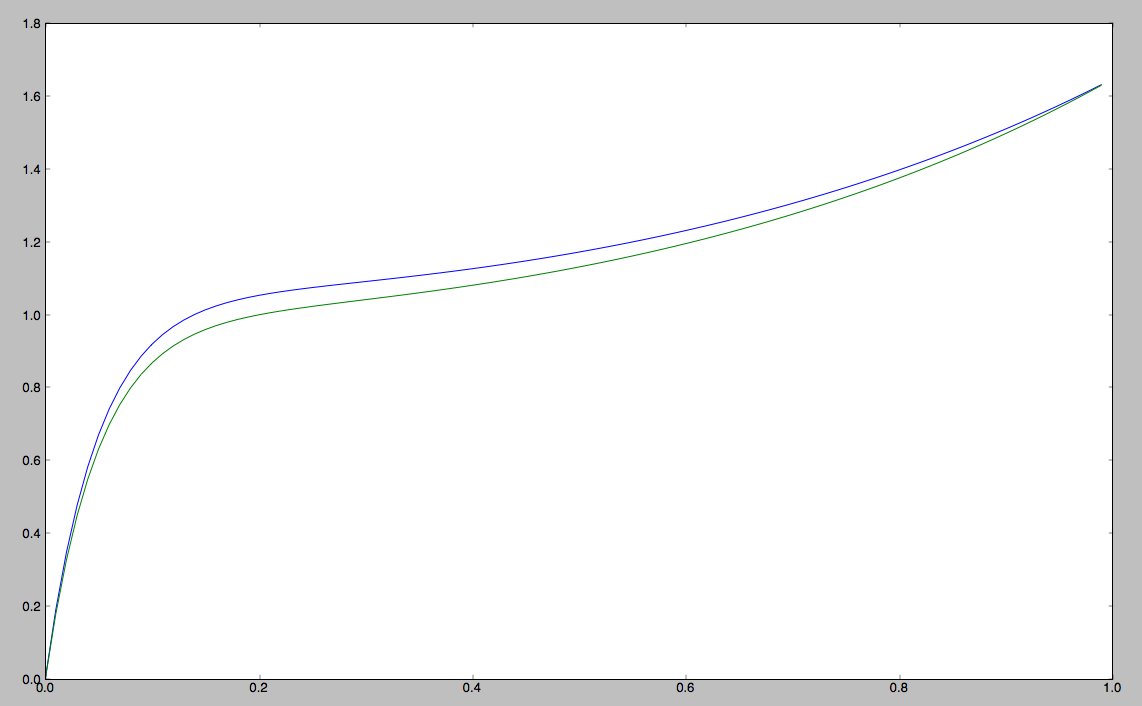
\includegraphics[angle=90,height=7in]{plot.png}
\caption{Plot of numerical results. Lower line is approximate solution.}
\end{center}
\end{figure}
\hfill $\blacksquare$
\item[Problem 4] We expand the ODE
\eqn{4ode}{
  \big[
  py'
  \big]'
  - ry
  =
  -\lam^2qy
}
\eqn{4ode_expand}{
  py'' + p'y' - py = -\lam^2 qy
}
Calculating
\eq{
  y &= hw\\
  y' &= h'w + hw'\\
  y'' &= h''w + 2 h'w' + hw''
}
Substituting these into \eqr{4ode_expand} yields
\eqn{4ode_subs}{
  ph''w + 2ph'w' + phw'' + p'h'w + p'hw' - rhw = -\lam^2qhw
}
Now to get the form we want, we need $w'$ to disappear, or
\eqn{4h_cond}{
  2ph' = p'h
  \qquad
  \implies
  \qquad
  \frac{h'}{h} = \frac{1}{2}\frac{p'}{p}
  \qquad
  \implies
  \qquad
  h = \frac{c}{\sqrt{p}}
}
Substituting \eqr{4h_cond} into \eqr{4ode_subs} and regrouping gives
\eqn{4ode_regroup}{
  pw'' + (
    \lam^2q
    - r
    + \frac{ph''}{h} 
    + \frac{p'h'}{h}
  )w = 0
}
Letting $
  f = 
  r
  - \frac{ph''}{h} 
  - \frac{p'h'}{h}
$ we find that
\eqn{4ode_f}{
  f = 
  \frac{1}{2} p'' 
  - \frac{1}{4} \frac{(p')^2}{p}
  + r
}
To find large eigenvalues, we let $\frac{1}{\lam} = \eps$ where $\eps$ is very small. Thus the $q$ term dominates in the $\lam^2 q - f$ term, reducing \eqr{4ode_regroup} to
\eqn{4ode_wkb}{
  \eps^2 pw'' = -qw
}
We apply a 1-term WKB approximation to \eqr{4ode_wkb} with $Q = -q/p$, and get
\eqn{4wkb_approx}{
  w =
  c_1 Q^{-1/4} e^{\frac{i}{\eps} \int_0^x \sqrt{Q}\; dt}
  +
  c_2 Q^{-1/4} e^{-\frac{i}{\eps} \int_0^x \sqrt{Q}\; dt}
}
Applying the boundary condition $w(0) = 0$ to \eqr{4wkb_approx} gives that $c_1 = -c_2$, so
\eqn{4wkb_approx_bc}{
  w = c_1 Q^{-1/4} \sin
  \big(
    \frac{1}{\eps} \int_0^x \sqrt{Q} \; dt
  \big)
}
If we define $\kappa = \int_0^1 \sqrt{Q} \; dt$ and apply the boundary condition $w(1) = 0$, we find
$$
  0 = c_1 Q^{-1/4}(1) \sin(\frac{\kappa}{\eps})
  \qquad
  \implies
  \qquad
  \frac{\kappa}{\eps} = n\pi
  \qquad
  \implies
  \qquad
  \lam_n = \frac{n\pi}{\kappa}
$$
So we find our eigenfunctions by plugging into \eqr{4wkb_approx_bc} and get
$$
  w_n = c_n Q^{-1/4} \sin(\lam_n x)
$$
$$
  y_n = d_n (pq)^{-1/4} \sin(\lam_n x)
$$
\hfill $\blacksquare$
\item[Problem 5]
We begin with
\eqn{pde}{
  u_t = u_xx + \lam u - u^3
}
Seeking a steady state solution, we drop the dependence on $t$ and get the ODE
\eqn{ode}{
  u_xx + \lam u - u^3 = 0
}
Seeking bifrucations from the steady state solution we let $\eps = \lam - \lam_b$ where $\lam_b$ is a lambda value corresponding to a bifrucation point.
We attempt to expand our solution as
$$
  u \sim u_s + \eps^\alpha u_1(x) + \eps^\beta u_2(x) + \ldots,
  \qquad
  0 < \alpha < \beta
$$
Substituting this expansion into \eqr{ode} gives
\eqn{expans}{
  \eps^\alpha(\p{x}^2 u_1 + \lam_b u_1)
  + \eps^\beta(\p{x}^2 u_2 + \lam_b u_2)
  + \eps^{1+\alpha} u_1
  + \eps^{3\alpha} u_1^3
  =
  0
}
The $O(\eps^\alpha)$ equation is given by
\eqn{u1_eqn}{
  \p{x}^2 u_1 + \lam_b u_1 = 0,
  \qquad
  u_1(0) = u_1(\pi) = 0
}
Solving \eqr{u1_eqn} yields
\eqn{u1_soln}{
  u_1
  =
  A_n \sin(n x),
  \qquad
  \lam_b = n^2
  ,
  n \in \mathbb{N}
}
Matching size of terms in the rest of \eqr{expans} we can see that the only choice that works is when
$$
  \alpha = \frac{1}{2}
  \qquad
  \beta = \frac{3}{2}
$$
In this case, we get an equation in $O(\eps^{3/2})$,
\eqn{u2_eqn}{
  \p{x}^2 u_2 + \lam_b u_2 = -u_1 - u_1^3,
  \qquad
  u_2(0) = u_2(\pi) = 0
}
By the Fredholm Alternative Theorem, we require that 
$$
  \langle
  u_1,
  -u_1 - u_1^3
  \rangle
  = 0
$$
or
\eqn{fred_req}{
  \int_0^\pi
  A_n^2 sin^2(nx)
  + A_n^4 sin^4(nx)
  \; dx
  = 0
}
To satisfy \eqr{fred_req} we must either have $A_n^2 = 0$ which is the trivial solution
or $A_n^2 = - \frac{4}{3}$. Substituting this back into \eqr{u1_soln}, we find
\eq{
  u_1 = \pm \frac{4}{3}i\sin(n x), \qquad n \in \mathbb{N}
}
Thus our bifrucating solutions are
\eqn{first_order}{
  u \sim
  \pm \sqrt{\eps} \frac{4}{3}i\sin(n x)
}

Carrying out the linearized stability analysis, we assume
\begin{eqnarray}
  u(x,0) &=& \delta g(x) \notag \\
  u_t(x,0) &=& \delta h(x) \notag \\
  u(x,t) &\sim& u_s + \delta v_1(x, t) + \ldots \label{linear_approx}\\
  \lambda &\neq& n^2 \notag
\end{eqnarray}
Substituting \eqr{linear_approx} into \eqr{pde} and drop higher order terms of $\delta$ to find
\eqn{v1_eqn}{
  \p{t}v_1
  =
  \p{x}^2 v_1 + \lambda v_1
}
with boundary/initial conditions
\begin{eqnarray}
  v_1(0) = v_1(\pi) = 0 \notag \\
  v_1(x,0) = g(x) \notag \\
  \p{t} v_1(x,0) = h(x) \notag
\end{eqnarray}
This can be solved by separation of variables. Let
$$
 v_1(x,t) = X(x)T(t)
$$
Then,
\eqn{X_soln}{
  X =
  c_1 e^{\sqrt{c - \lambda} x}
  + c_2 e^{-\sqrt{c - \lambda} x}
}
\eqn{T_soln}{
  T = e^{ct} + d
}
Applying boundary/initial conditions to \eqr{X_soln} and \eqr{T_soln}
and summing up all the linearly independent solutions gives
\eqn{v1_soln}{
  v_1(x,t) = \sum_{n=1}^\infty
  \bigg(
    e^{(n^2 + \lambda) t} + a_n
  \bigg)
  b_n \sin(nx)
}
Thus, the solution is unstable for all values of $\lambda$ unless the coeffcients
$b_n$ are all zero for $n > N$, then if $-\lam > N^2$, we have stability. We do not
need to consider stability at the bifrucation point because this condition is not
sensitive to small changes in $\lam$.
\hfill $\blacksquare$
\end{description}
\end{document}
